\documentclass{article}
\usepackage[margin=1in]{geometry}
\usepackage[linesnumbered,ruled,vlined]{algorithm2e}
\usepackage{amsfonts}
\usepackage{amsmath}
\usepackage{amssymb}
\usepackage{amsthm}
\usepackage{enumitem}
\usepackage{fancyhdr}
\usepackage{hyperref}
\usepackage{minted}
\usepackage{multicol}
\usepackage{pdfpages}
\usepackage{standalone}
\usepackage[many]{tcolorbox}
\usepackage{tikz-cd}
\usepackage{transparent}
\usepackage{xcolor}
% \tcbuselibrary{minted}

\author{Nathan Solomon}

\newcommand{\fig}[1]{
    \begin{center}
        \includegraphics[width=\textwidth]{#1}
    \end{center}
}

% Math commands
\renewcommand{\d}{\mathrm{d}}
\DeclareMathOperator{\id}{id}
\DeclareMathOperator{\im}{im}
\DeclareMathOperator{\proj}{proj}
\DeclareMathOperator{\Span}{span}
\DeclareMathOperator{\Tr}{Tr}
\DeclareMathOperator{\tr}{tr}
\DeclareMathOperator{\ad}{ad}
\DeclareMathOperator{\ord}{ord}
%%%%%%%%%%%%%%% \DeclareMathOperator{\sgn}{sgn}
\DeclareMathOperator{\Aut}{Aut}
\DeclareMathOperator{\Inn}{Inn}
\DeclareMathOperator{\Out}{Out}
\DeclareMathOperator{\stab}{stab}

\newcommand{\N}{\ensuremath{\mathbb{N}}}
\newcommand{\Z}{\ensuremath{\mathbb{Z}}}
\newcommand{\Q}{\ensuremath{\mathbb{Q}}}
\newcommand{\R}{\ensuremath{\mathbb{R}}}
\newcommand{\C}{\ensuremath{\mathbb{C}}}
\renewcommand{\H}{\ensuremath{\mathbb{H}}}
\newcommand{\F}{\ensuremath{\mathbb{F}}}

\newcommand{\E}{\ensuremath{\mathbb{E}}}
\renewcommand{\P}{\ensuremath{\mathbb{P}}}

\newcommand{\es}{\ensuremath{\varnothing}}
\newcommand{\inv}{\ensuremath{^{-1}}}
\newcommand{\eps}{\ensuremath{\varepsilon}}
\newcommand{\del}{\ensuremath{\partial}}
\renewcommand{\a}{\ensuremath{\alpha}}

\newcommand{\abs}[1]{\ensuremath{\left\lvert #1 \right\rvert}}
\newcommand{\norm}[1]{\ensuremath{\left\lVert #1\right\rVert}}
\newcommand{\mean}[1]{\ensuremath{\left\langle #1 \right\rangle}}
\newcommand{\floor}[1]{\ensuremath{\left\lfloor #1 \right\rfloor}}
\newcommand{\ceil}[1]{\ensuremath{\left\lceil #1 \right\rceil}}
\newcommand{\bra}[1]{\ensuremath{\left\langle #1 \right\rvert}}
\newcommand{\ket}[1]{\ensuremath{\left\lvert #1 \right\rangle}}
\newcommand{\braket}[2]{\ensuremath{\left.\left\langle #1\right\vert #2 \right\rangle}}

\newcommand{\catname}[1]{{\normalfont\textbf{#1}}}

\newcommand{\up}{\ensuremath{\uparrow}}
\newcommand{\down}{\ensuremath{\downarrow}}

% Custom environments
\newtheorem{thm}{Theorem}[section]

\definecolor{probBackgroundColor}{RGB}{250,240,240}
\definecolor{probAccentColor}{RGB}{140,40,0}
\newenvironment{prob}{
    \stepcounter{thm}
    \begin{tcolorbox}[
        boxrule=1pt,
        sharp corners,
        colback=probBackgroundColor,
        colframe=probAccentColor,
        borderline west={4pt}{0pt}{probAccentColor},
        breakable
    ]
    \color{probAccentColor}\textbf{Problem \thethm.} \color{black}
} {
    \end{tcolorbox}
}

\definecolor{exampleBackgroundColor}{RGB}{212,232,246}
\newenvironment{example}{
    \stepcounter{thm}
    \begin{tcolorbox}[
      boxrule=1pt,
      sharp corners,
      colback=exampleBackgroundColor,
      breakable
    ]
    \textbf{Example \thethm.}
} {
    \end{tcolorbox}
}

\definecolor{propBackgroundColor}{RGB}{255,245,220}
\definecolor{propAccentColor}{RGB}{150,100,0}
\newenvironment{prop}{
    \stepcounter{thm}
    \begin{tcolorbox}[
        boxrule=1pt,
        sharp corners,
        colback=propBackgroundColor,
        colframe=propAccentColor,
        breakable
    ]
    \color{propAccentColor}\textbf{Proposition \thethm. }\color{black}
} {
    \end{tcolorbox}
}

\definecolor{thmBackgroundColor}{RGB}{235,225,245}
\definecolor{thmAccentColor}{RGB}{50,0,100}
\renewenvironment{thm}{
    \stepcounter{thm}
    \begin{tcolorbox}[
        boxrule=1pt,
        sharp corners,
        colback=thmBackgroundColor,
        colframe=thmAccentColor,
        breakable
    ]
    \color{thmAccentColor}\textbf{Theorem \thethm. }\color{black}
} {
    \end{tcolorbox}
}

\definecolor{corBackgroundColor}{RGB}{240,250,250}
\definecolor{corAccentColor}{RGB}{50,100,100}
\newenvironment{cor}{
    \stepcounter{thm}
    \begin{tcolorbox}[
        enhanced,
        boxrule=0pt,
        frame hidden,
        sharp corners,
        colback=corBackgroundColor,
        borderline west={4pt}{0pt}{corAccentColor},
        breakable
    ]
    \color{corAccentColor}\textbf{Corollary \thethm. }\color{black}
} {
    \end{tcolorbox}
}

\definecolor{lemBackgroundColor}{RGB}{255,245,235}
\definecolor{lemAccentColor}{RGB}{250,125,0}
\newenvironment{lem}{
    \stepcounter{thm}
    \begin{tcolorbox}[
        enhanced,
        boxrule=0pt,
        frame hidden,
        sharp corners,
        colback=lemBackgroundColor,
        borderline west={4pt}{0pt}{lemAccentColor},
        breakable
    ]
    \color{lemAccentColor}\textbf{Lemma \thethm. }\color{black}
} {
    \end{tcolorbox}
}

\definecolor{proofBackgroundColor}{RGB}{255,255,255}
\definecolor{proofAccentColor}{RGB}{80,80,80}
\renewenvironment{proof}{
    \begin{tcolorbox}[
        enhanced,
        boxrule=1pt,
        sharp corners,
        colback=proofBackgroundColor,
        colframe=proofAccentColor,
        borderline west={4pt}{0pt}{proofAccentColor},
        breakable
    ]
    \color{proofAccentColor}\emph{\textbf{Proof. }}\color{black}
} {
    \qed \end{tcolorbox}
}

\definecolor{noteBackgroundColor}{RGB}{240,250,240}
\definecolor{noteAccentColor}{RGB}{30,130,30}
\newenvironment{note}{
    \begin{tcolorbox}[
        enhanced,
        boxrule=0pt,
        frame hidden,
        sharp corners,
        colback=noteBackgroundColor,
        borderline west={4pt}{0pt}{noteAccentColor},
        breakable
    ]
    \color{noteAccentColor}\textbf{Note. }\color{black}
} {
    \end{tcolorbox}
}


\fancyhf{}
\setlength{\headheight}{24pt}

\date{\today}
\title{Physics 245 Homework \#2}

\begin{document}
\maketitle

\begin{prob}
\end{prob}
\begin{enumerate}[label=(\alph*)]
    \item
        \[ H = -\mu \cdot B = \frac{g\mu_B}{\hbar} S \cdot B = \frac{g\mu_B}{2} B \cdot \sigma = \frac{g\mu_B}{2} \begin{bmatrix}
            B_z & B_x \\
            B_x & -B_z
        \end{bmatrix} \]
        To find the eigenvalues, we set the characteristic polynomial $\det (H-\lambda I)$ equal to zero.
        \begin{align*}
            0 &= \left( \frac{g\mu_BB_z}{2} - \lambda \right) \left( - \frac{g\mu_BB_z}{2} - \lambda \right) - \left( \frac{g\mu_BB_x}{2} \right)^2 \\
              &= \lambda^2 - \left( \frac{g\mu_B}{2} \right)^2 (B_z^2 + B_x^2) \\
            \lambda &= \pm \frac{g\mu_B}{2} \sqrt{B_z^2 + B_x^2}
        \end{align*}
        So the corresponding eigenvectors are vectors in the nullspace of
        \[ \frac{g\mu_B}{2} \begin{bmatrix}
            B_z \mp \sqrt{B_z^2 + B_x^2} & B_x \\
            B_x & -B_z \mp \sqrt{B_z^2 + B_x^2}
        \end{bmatrix}. \]
        For the positive eigenvalue, the eigenbasis is spanned by the vector
        \[ \begin{bmatrix}
            1 \\
            - B_z/B_x + \sqrt{1 + B_z^2/B_x^2}
        \end{bmatrix} \]
        and for the negative eigenvalue, the eigenbasis is spanned by
        \[ \begin{bmatrix}
            1 \\
            - B_z/B_x - \sqrt{1 + B_z^2/B_x^2}
        \end{bmatrix}. \]
        I will not bother normalizing the eigenvectors yet, because that would be unnecessarily ugly.
    \item If $B_z >> B_x$, then the positive eigenvalue is $\approx \frac{g\mu_B}{2} B_z$, and its corresponding eigenvector is $\approx \begin{bmatrix}
            1 \\
            0
        \end{bmatrix}$.
        The negative eigenvalue is $\approx - \frac{g\mu_B}{2} B_z$, and its corresponding eigenvector (up to a constant) is $ \approx \begin{bmatrix}
            0 \\
            1
        \end{bmatrix}$.
    \item If $B_x >> B_z$, then the positive eigenvalue is $\approx \frac{g\mu_B}{2} B_x$, and its corresponding eigenvector is $\approx \begin{bmatrix}
            1 \\
            1
        \end{bmatrix}$.
        The negative eigenvalue is $\approx - \frac{g\mu_B}{2} B_x$, and its corresponding eigenvector is $ \approx \begin{bmatrix}
            1 \\
            -1
        \end{bmatrix}$. Both of these eigenvectors could be normalized by just dividing by $\sqrt{2}$.
    \item Let $\hat{z'}$ be a unit vector pointing in the direction of the magnetic field $B$. Then
        \[ \hat{z'} = \frac{B_x \hat{x} + B_z \hat{z}}{\sqrt{B_x^2 + B_z^2}}. \]
        Just like $\sigma_z = \sigma \cdot \hat{z}$ and $\sigma_x = \sigma \cdot \hat{x}$,
        we can define $\sigma_{\hat{z'}}$ to be
        \[ \sigma_{\hat{z'}} = \frac{B_x\sigma_x+B_z\sigma_z}{\sqrt{B_x^2+B_z^2}} = \frac{1}{\sqrt{B_x^2+B_z^2}} \begin{bmatrix}
            B_z & B_x \\
            B_x & -B_z
        \end{bmatrix}, \]
        which can be factored out of the expression I found in part (a) for the Hamiltonian:
        \[ H = A \sigma_{\hat{z'}} = \frac{g\mu_B \sqrt{B_x^2+B_z^2}}{2} \sigma_{\hat{z'}}. \]
        Here, $A$ is a scalar (or a scalar times the identity matrix, but that wouldn't be interesting), so I will assume the question is asking for the eigenvalues and eigenvectors of $H$. But those are exactly the same as they were in part (a). The eigenvalues of $\sigma_{\hat{z'}}$ are $\pm 1$ and the eigenvectors of $\sigma_{\hat{z'}}$ are the same as the eigenvectors of $H$. The direction of the new $z'$ axis is
        \[ \hat{z'} = \operatorname{unit}(B) = \frac{B_x \hat{x} + B_z\hat{z}}{\sqrt{B_x^2+B_z^2}}. \]
    \item The (normalized) positive energy eigenstate is
        \[ \frac{1}{\sqrt{2 + 2Bz^2/B_x^2-2B_z/B_x \sqrt{1+B_z^2/B_x^2}}} \cdot \begin{bmatrix}
            1 \\
            -B_z/B_x + \sqrt{1+B_z^2/B_x^2}
        \end{bmatrix} \]
        So the expected value of spin along the $z$-axis is $\hbar/2$ times the first component squared, plus $-\hbar/2$ times the second component squared:
        \begin{align*}
            \mean{S} &= \frac{\hbar}{2} \left( \frac{1}{2+2 \frac{B_z^2}{B_x^2}- 2 \frac{B_z}{B_x} \sqrt{1+ \frac{B_z^2}{B_x^2}}} \right) - \frac{\hbar}{2} \left( \frac{ 1 + 2\frac{B_z^2}{B_x^2} - 2 \frac{B_z}{B_x} \sqrt{1 + \frac{B_z^2}{B_x^2}}}{2+2 \frac{B_z^2}{B_x^2}- 2 \frac{B_z}{B_x} \sqrt{1+ \frac{B_z^2}{B_x^2}}} \right) 
        \end{align*}
        I didn't want to convert that from \LaTeX to whatever format Wolfram Alpha uses, so I used ChatGPT to simplify that expression. The result was
        \[ \mean{S} = \frac{\hbar}{2} \left( \frac{- \frac{B_z^2}{B_x^2} + \frac{B_z}{B_x} \sqrt{1 + \frac{B_z^2}{B_x^2}}}{1 + \frac{B_z^2}{B_x^2} - \frac{B_z}{B_x} \sqrt{1 + \frac{B_z^2}{B_x^2}}} \right). \]
\end{enumerate}


\bigskip
\begin{prob}
\end{prob}
See the jupyter notebook a few pages below this.

\bigskip
\begin{prob}
\end{prob}
I used QuTiP to calculate these, because it would be tedious to do by hand. For each of the Pauli spin matrices, the eigenvalues are $\pm 1$.
\begin{enumerate}[label=(\alph*)]
    \item The $\lambda=-1$ eigenvector is $\frac{1}{\sqrt{2}} \begin{bmatrix}
        -1 \\
        1
\end{bmatrix}$ and the $\lambda=+1$ eigenvector is $\frac{1}{\sqrt{2}} \begin{bmatrix}
    1 \\
    1
\end{bmatrix}$.
    \item The $\lambda=-1$ eigenvector is $\frac{1}{\sqrt{2}} \begin{bmatrix}
        -1 \\
        i
\end{bmatrix}$ and the $\lambda=+1$ eigenvector is $\frac{1}{\sqrt{2}} \begin{bmatrix}
    1 \\
    i
\end{bmatrix}$.
    \item The $\lambda=-1$ eigenvector is $\begin{bmatrix}
        0 \\
        1
\end{bmatrix}$ and the $\lambda=+1$ eigenvector is $\begin{bmatrix}
    1 \\
    0
\end{bmatrix}$.
\end{enumerate}


\bigskip
\begin{prob}
\end{prob}
\begin{enumerate}[label=(\alph*)]
    \item
        \[ \sigma_x^2 = \begin{bmatrix}
            0 & 1 \\
            1 & 0
        \end{bmatrix}^2 = I \]
    \item
        \[ \sigma_y^2 = \begin{bmatrix}
            0 & -i \\
            i & 0
        \end{bmatrix}^2 = I \]
    \item
        \[ \sigma_z^2 = \begin{bmatrix}
            1 & 0 \\
            0 & -1
        \end{bmatrix}^2 = I \]
    \item
        \begin{align*}
            \exp(i\theta \sigma_x) &= \left( I + \frac{i\theta}{1!} \sigma_x + \frac{i^2\theta^2}{2!} I + \frac{i^3\theta^3}{3!} \sigma_x + \cdots \right) \\
                                   &= \cos(\theta) \cdot I + i \sin(\theta) \cdot \sigma_x \\
                                   &= \begin{bmatrix}
                                       \cos \theta & i \sin \theta \\
                                       i \sin \theta & \cos \theta
                                   \end{bmatrix}
        \end{align*}
    \item
        \begin{align*}
            \exp(i\theta \sigma_y) &= \left( I + \frac{i\theta}{1!} \sigma_y + \frac{i^2\theta^2}{2!} I + \frac{i^3\theta^3}{3!} \sigma_y + \cdots \right) \\
                                   &= \cos(\theta) \cdot I + i \sin(\theta) \cdot \sigma_y \\
                                   &= \begin{bmatrix}
                                       \cos \theta & \sin \theta \\
                                       - \sin \theta & \cos \theta
                                   \end{bmatrix}
        \end{align*}
    \item
        \[ \exp(i \theta \sigma_z) = \exp \left( \begin{bmatrix}
                i \theta & 0 \\
                0 & -i \theta
        \end{bmatrix} \right) = \begin{bmatrix}
                e^{i\theta} & 0 \\
                0 & e^{-i\theta}
        \end{bmatrix} \]
        
        
\end{enumerate}

\bigskip
\begin{prob}
\end{prob}
Apply a time-dependent magnetic field to an electron spin state, so that the hamiltonian is
\[ H = \mu_B B_z \sigma_z + \mu_B B_x \cos (\omega t + \phi) \sigma_x. \]
Then we can define $\Omega := \mu_B B_x / \hbar$ to be the Rabi frequency, $\omega_0 := 2 \mu_B B_z / \hbar$ to be the qubit frequency, and $\delta := \omega - \omega_0$ to be the detuning. Assume $\phi=0$. Then
\[ \frac{H}{\hbar} = \frac{\omega_0}{2} \sigma_z + \Omega \cos (\omega t) \sigma_x = \begin{bmatrix}
    \omega_0/2 & \Omega \cos (\omega t) \\
    \Omega \cos (\omega t) & -\omega_0 / 2
\end{bmatrix}. \]
We can plug that Hamiltonian into the Schrödinger equation and guess that the solution will have the form
\[ \ket{\Psi} = \begin{bmatrix}
    a \exp \left( -i \omega_0 t / 2 \right) \\
    b \exp \left( i \omega_0 t / 2 \right)
\end{bmatrix}, \]
where $a, b \in \C$ may depend on time. The Schrödinger equation for our qubit is
\[  \frac{\partial}{\partial t} \ket{\Psi} = i \frac{\partial}{\partial t} \begin{bmatrix}
    a \\
    b
\end{bmatrix} = \begin{bmatrix}
    \omega_0/2 & \Omega \cos (\omega t) \\
    \Omega \cos (\omega t) & -\omega_0 / 2
\end{bmatrix} \begin{bmatrix}
    a \\
    b
\end{bmatrix} = H \ket{\Psi}. \]
From that, we get two coupled differential equations for $a$ and $b$:
\begin{align*}
    i \dot{a} &= b e^{i \omega_0 t} \Omega \cos(\omega t) \\
    i \dot{b} &= a e^{- i \omega_0 t} \Omega \cos(\omega t).
\end{align*}
At this point, we will assume $\omega + \omega_0 >> \Omega$, but the driving frequency is probably close to the qubit frequency, so we cannot assume $\delta = \omega - \omega_0 >> \Omega$. This is relevant because we can now make the rotating wave approximation:
\begin{align*}
    i \dot{a} &= b e^{i \omega_0 t} \Omega \frac{e^{i \omega t} + e^{-i \omega t}}{2} \approx \frac{\Omega b}{2} e^{-i \delta t} \\
    i \dot{b} &= a e^{- i \omega_0 t} \Omega \frac{e^{i \omega t} + e^{-i \omega t}}{2} \approx \frac{\Omega a}{2}e^{i \delta t}.
\end{align*}
Now we can use substitution to uncouple these equations:
\begin{align*}
    i \ddot{a} &= \frac{\partial}{\partial t} \left( \frac{\Omega b}{2} e^{-i \delta t} \right) \\
               &= \frac{\Omega}{2} \dot{b}e^{-i \delta t} - \frac{\Omega}{2} i \delta b e^{-i \delta t} \\
               &= \frac{\Omega^2}{4i} a - i \delta (i \dot{a}) \\
    0 &= \ddot{a} + i \delta \dot{a} + \frac{\Omega^2}{4} a.
\end{align*}
Guess that the fundamental set of solutions is $a \in \Span \left\{ e^{\lambda_- t}, e^{\lambda_+ t} \right\}$, where $\lambda_\pm$ are roots of the following quadratic equation:
\begin{align*}
    0 &= \lambda^2 e^{\lambda t} + i \delta \lambda e^{\lambda t} + \frac{\Omega^2}{4} e^{\lambda t} \\
    0 &= \lambda^2 + i \delta \lambda + \frac{\Omega^2}{4} \\
    \lambda &= \frac{-i\delta \pm \sqrt{-\delta^2 - \Omega^2}}{2} \\
    \lambda_- :&= \frac{-i\delta -i \Omega'}{2} \\
    \lambda_+ :&= \frac{-i\delta + i \Omega'}{2}
\end{align*}
Since we are given that $\ket{\Psi}=\ket{0}$ at time $t=0$, we know $a=1$ and $b=0$ at $t=0$, which means $\dot{a}=0$ at $t=0$.
\begin{align*}
    a &= C_1 e^{\lambda_- t}+C_2 e^{\lambda_+ t} \\
    a(t=0) &= C_1+C_2 \\
    \dot{a}(t=0) &= 0 = \lambda_- C_1 + \lambda_+ C_2 \\
    \begin{bmatrix}
        C_1 \\
        C_2
    \end{bmatrix} &= \begin{bmatrix}
    1 & 1 \\
    \frac{i}{2} (-\delta -\Omega') & \frac{i}{2} (-\delta + \Omega')
\end{bmatrix}^{-1} \begin{bmatrix}
    1 \\
    0
\end{bmatrix} = \begin{bmatrix}
\frac{1}{2} \left( 1 - \frac{\delta}{\Omega'} \right) \\
\frac{1}{2} \left( 1 + \frac{\delta}{\Omega'} \right) 
\end{bmatrix} \\
    a &= \left( \frac{1}{2} - \frac{\delta}{2\Omega'} \right) \exp \left( \frac{-i \delta - i \Omega'}{2} t \right) + \left( \frac{1}{2} + \frac{\delta}{2\Omega'} \right) \exp \left( \frac{-i \delta + i \Omega'}{2} t \right) \\
      &= \exp (-i\delta t/ 2) \left( \cos \left( \frac{\Omega't}{2} \right) + \frac{i\delta}{\Omega'} \sin \left( \frac{\Omega't}{2} \right)  \right) 
\end{align*}
The probability of being in state $\ket{0}$ is
\begin{align*}
    P_0 = a^*a &= \cos^2 \left( \frac{\Omega't}{2} \right) + \frac{\delta^2}{\Omega'^2} \sin^2 \left( \frac{\Omega't}{2} \right) \\
               &= 1 - \left( 1 - \frac{\delta^2}{\Omega'^2} \right) \sin^2 \left( \frac{\Omega't}{2} \right) \\
               &= 1 - \frac{\Omega^2}{\Omega'^2} \sin^2 \left( \frac{\Omega't}{2} \right).
\end{align*}
If $\Omega t = \pi$, then $P_1 = 1 - P_0$ can be written as a function of only $\delta$ (and $\Omega$, which is a constant):
\begin{align*}
    P_1 &= \frac{\Omega^2}{\Omega^2 + \delta^2} \sin^2 (\pi/2) \\
        &= \frac{\Omega^2}{\Omega^2 + \delta^2}.
\end{align*}
See the jupyter notebook below for a plot of this function.

\bigskip
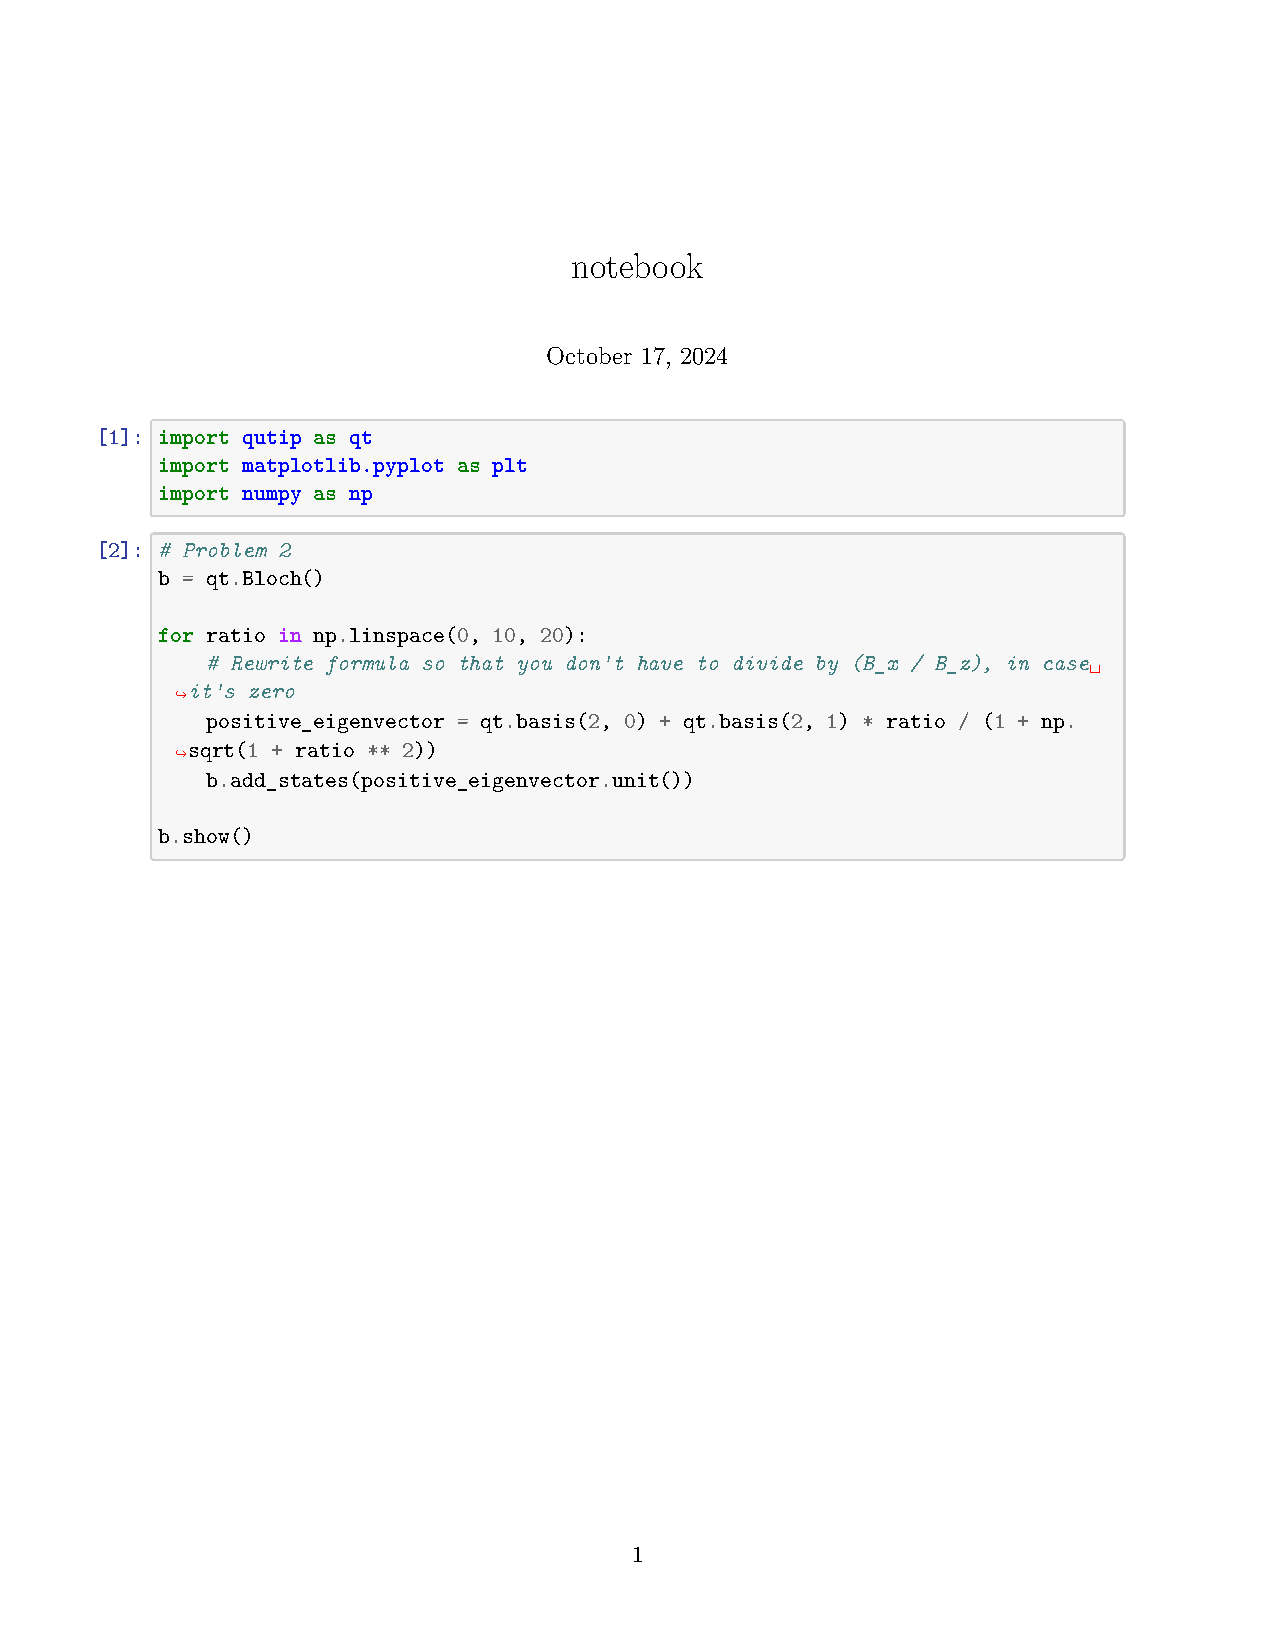
\includepdf[pages=-]{notebook.pdf}
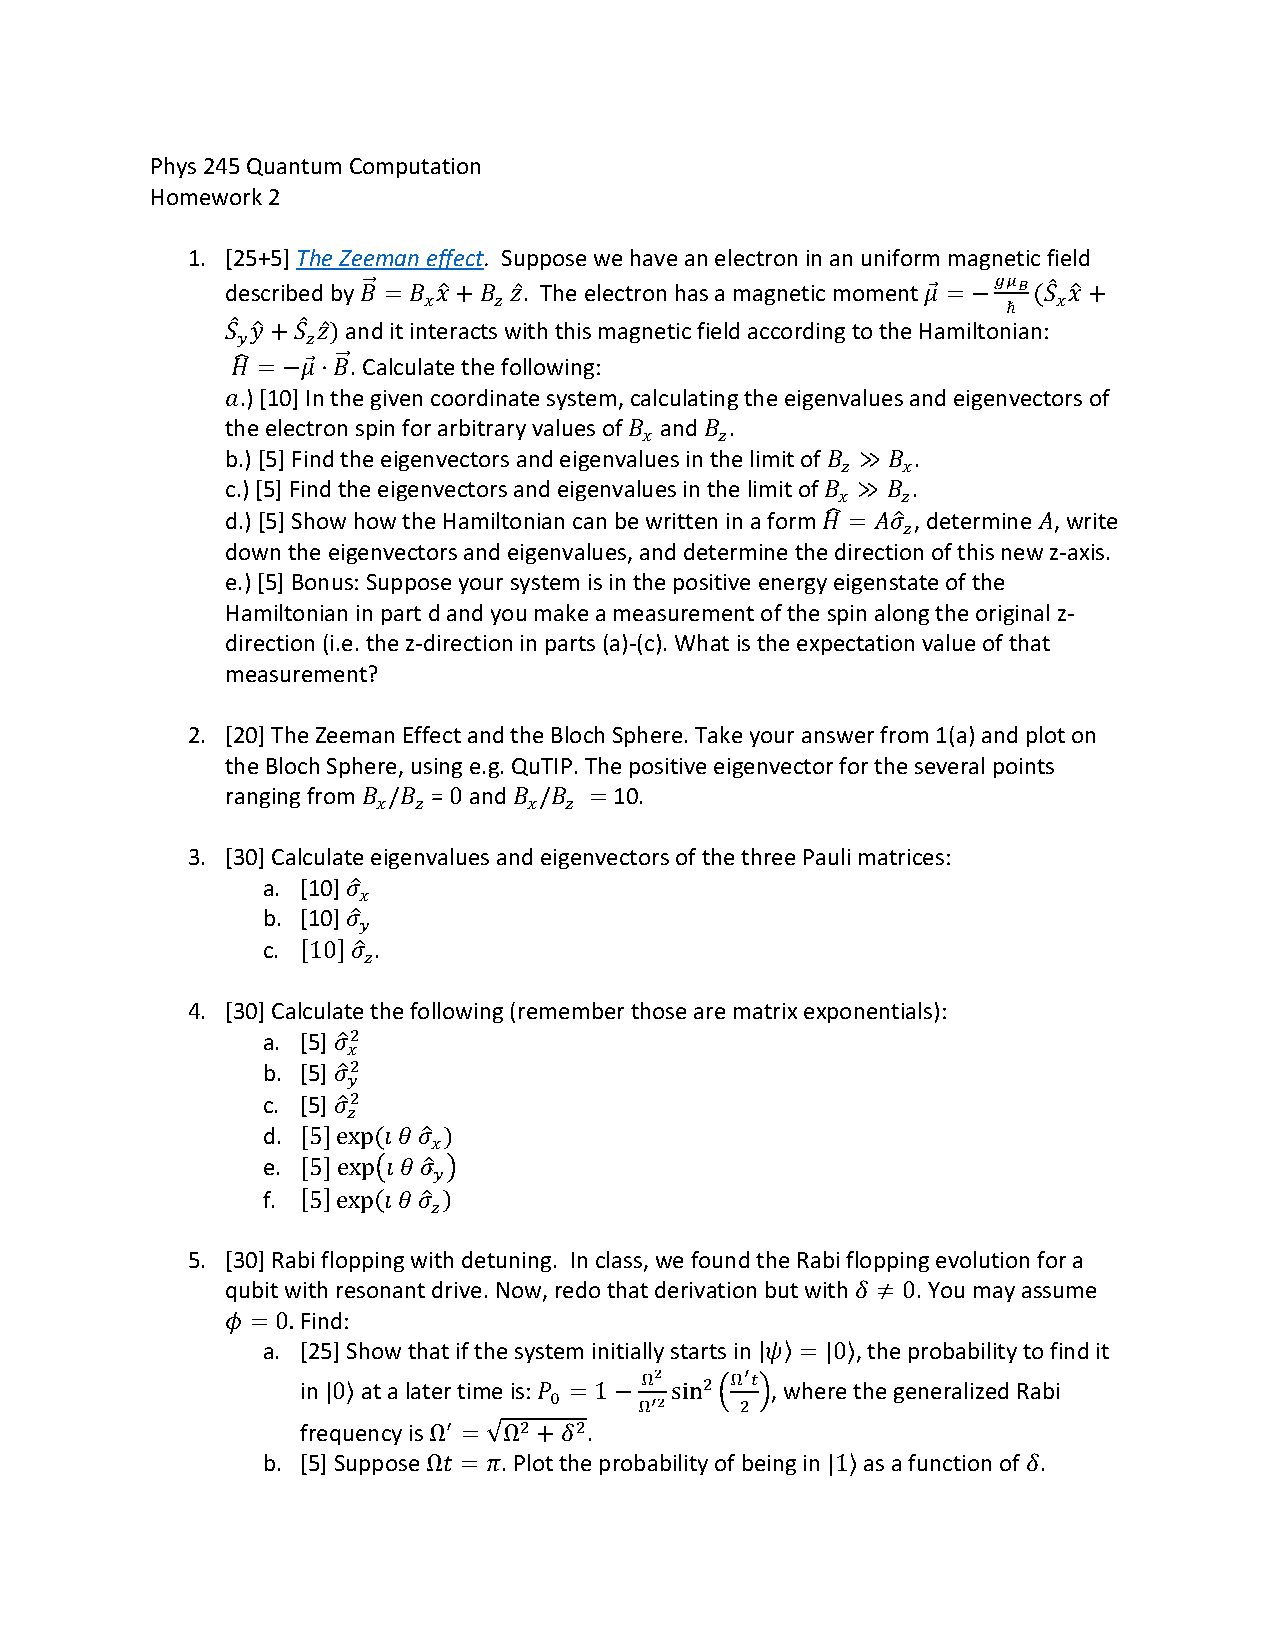
\includepdf[pages=-]{assignment.pdf}

\end{document}
